\chapter{Kajian Pustaka}

\section{ECG dan PPG}
Terdapat 2 jenis sensor yang umum digunakan untuk melakukan monitoring jantung, yaitu \textit{Electrocardiogram} (ECG) dan \textit{Photoplethysmogram} (PPG) seperti yang terlihat pada gambar \ref{fig:ecg_n_ppg}. Kedua jenis sensor ini menjadi pilihan utama dalam monitoring jantung karena keduanya mengusung konsep \textit{non-invasive}. Sensor non-invasive memungkinkan melakukan pengambilan data tubuh tanpa perlu melukai/menusuk bagian tubuh tertentu. Secara umum ECG akan menghasilkan pengukuran lebih akurat dari pada PPG. Namun PPG lebih nyaman digunakan dalam jangka panjang dari pada ECG.

\begin{figure}[h!]
    \centering
    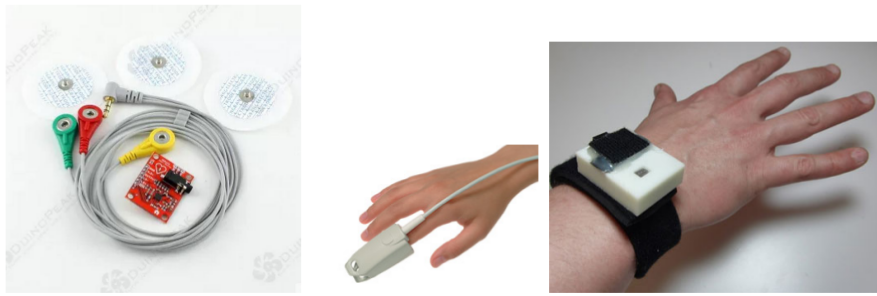
\includegraphics[scale=0.3]{images/sensors.png}
    \caption{a. Sensor ECG dengan 3 titik timbal, b. Sensor PPG ujung jari, c. Sensor PPG di pergelangan tangan}
    \label{fig:ecg_n_ppg}
\end{figure}

\subsection{Pembacaan Sinyal}
Walaupun kedua jenis sensor dapat digunakan untuk monitor jantung, sinyal yang dihasilkan sedikit berbeda, terlihat pada gambar \ref{fig:ecg_vs_ppg} \cite{ppg_vs_ecg}. Secara langsung dapat dilihat sinyal hasil dari PPG dengan ECG berbeda secara morfologi (bentuk). Karena sumber sinyal yang sama (dari jantung) siklus PPG dan ECG juga sama sehingga kedua sinyal dapat disinkronisasi (saling dipetakan) berdasarkan waktu seperti gambar \ref{fig:ecg_vs_ppg2} \cite{ecg_syncro}.
\begin{figure}[h!]
    \centering
    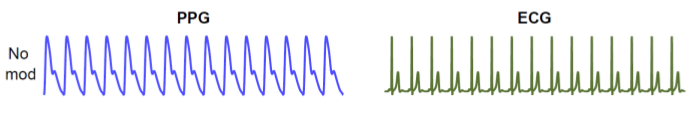
\includegraphics[scale=0.5]{images/ecg_vs_ppg.png}
    \caption{Perbandingan sinyal PPG dan ECG (ideal, dan termodulasi)}
    \label{fig:ecg_vs_ppg}
    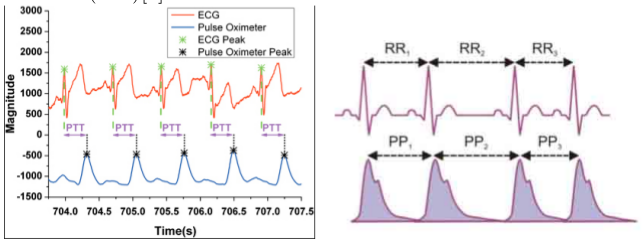
\includegraphics[scale=0.5]{images/similarity.png}
    \caption{Sinkronisasi antara ECG dan PPG}
    \label{fig:ecg_vs_ppg2}
\end{figure}

\section{Aritmia}